\section{Interrogations}

\subsection{Neural OP vs Diffusion Models : what's going on and where do we stand ?}

\noindent Neural Operators are:
\begin{itemize}
    \item Solving PDEs (and ODEs)
    \item Able to forecast the entire trajectory in 1 forward pass
    \item Using Spectral Conv
    \item Evaluated on datasets such as Navier-Strokes, Burgers, Poisson, ...
\end{itemize}

\noindent Diffusion Models are:
\begin{itemize}
    \item Sampling images and video
    \item Multi-step denoising
    \item Enforcing the Consistency Property that leads to Self-training
    \item Evaluated on datasets such as Cifar-10, Imagenet, ...
\end{itemize}

\begin{figure}[htbp]
  \centering
    \begin{tabular}{cc}
  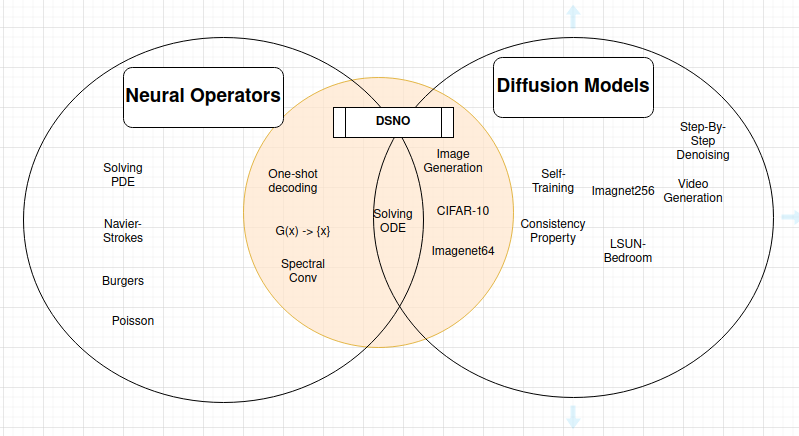
\includegraphics[width=0.5\textwidth]{figures/brainstorming.png} & 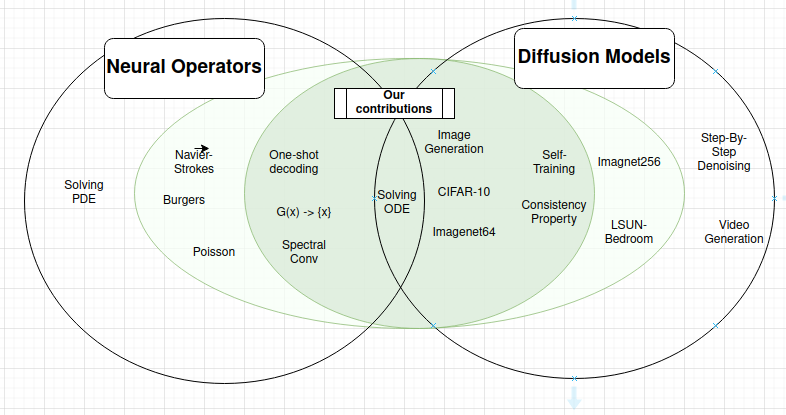
\includegraphics[width=0.5\textwidth]{figures/brainstorming2.png} \\
  \end{tabular}
  \caption{Current State of the Art in Neural OP vs Diffusion Models. Left figure describe how DSNO \cite{zheng2023fastsamplingdiffusionmodels} bridges the gap between NO and DM. Right figure show what we plan to build upon DSNO : enforcing the Consistency Property so that we can perform self-training, and then later extending experiments to datasets from both fields.}
  \label{fig:genno}
\end{figure}

\subsection{Plan of attack}

\begin{enumerate}
    \item Import/recode DSNO
    \item Test it on "fake data" or NO data
    \item Implement Self-Training for DSNO
    \item Test it on CIFAR/IMAGENET 64
    \item Implement SpectralConv with Temporal embedings)
    \item Then our version of DSNO fully treats time embeding (check with consistency models code)
    \item Try other Image datasets (IMAGENET 256, LSUN)
    \item Try other NO data/sets (Burgers, Poissons, Navier Strokes)
\end{enumerate}

\subsection{Background Information}
DSNO = Diffusion Model Architecture, with Neural Operator blocks that are part of the architecture. 

\begin{figure}[htbp]
  \centering
  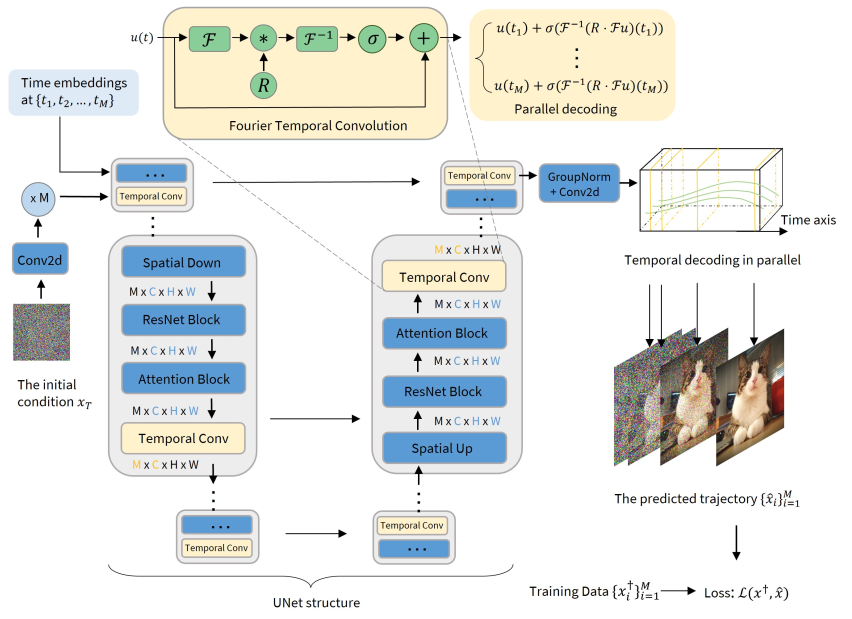
\includegraphics[width=0.75\textwidth]{figures/dsno.png}
  \caption{The DSNO architecture. The blue blocks form a classic U-Net shaped diffusion model (stacks of Spatial Downgrading/Upgrading + Residual Layer + Attention Blocks), while the yellow blocks are SpectralConvolution layers imported from Neural Operators.}
  \label{fig:genno}
\end{figure}

\begin{figure}[htbp]
  \centering
  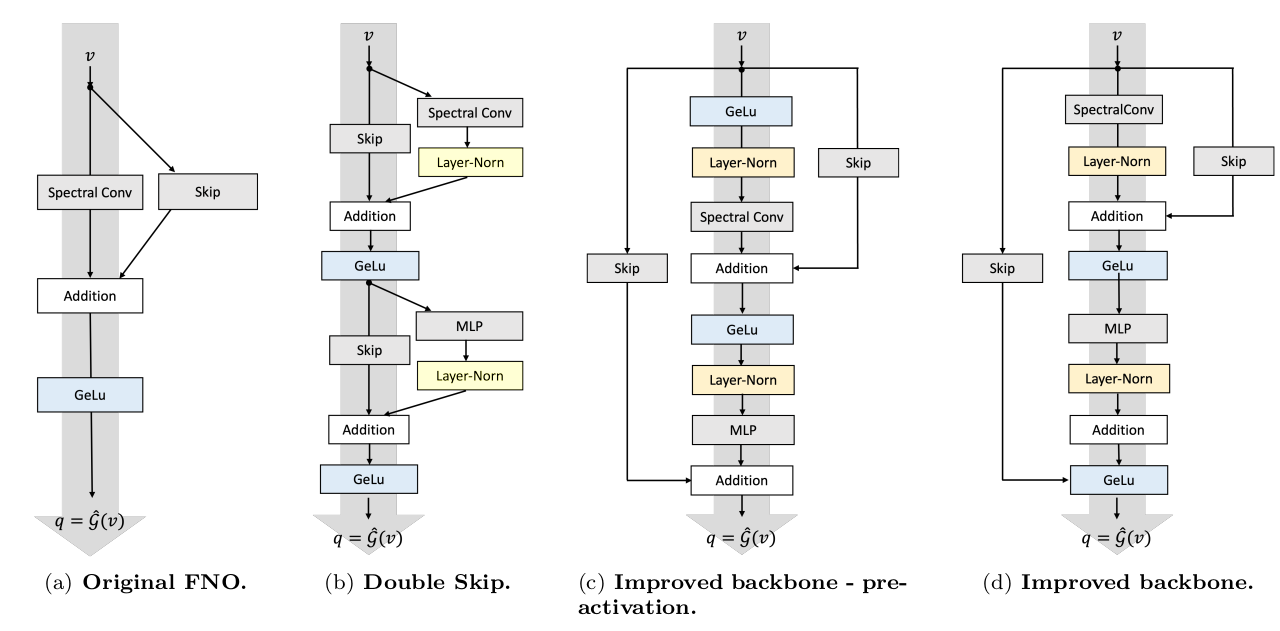
\includegraphics[width=0.75\textwidth]{figures/fno.png}
  \caption{Different FNO blocks architectures.}
  \label{fig:genno}
\end{figure}

\subsubsection{What makes diffusion models "Self-trainable ?"}
\begin{itemize}
    \item The Consistency Property 
    \item The noising process definition : $\x_{t_n} = \x + t_nz$ + \cite{song2023consistencymodels}'s Theorem 2 that we adapt to $\G$ in Appendix~\ref{app:loss}
\end{itemize}